\documentclass[onecolumn]{article}
\usepackage{graphicx}
\usepackage{float}
\usepackage{amsmath}
\usepackage{hyperref}
\restylefloat{figure}
\begin{document}

\title{Filling space with coloured cubes}

\author{Arjen Markus}

\maketitle

\section*{The question: three or more colours?}
Using cubes with two different colours you can easily fill three-dimensional space
in an elegant way, that is, the cubes of the same colour are all connected, the
distribution is in a sense uniform and isotropic and the cubes of the same colour are
equal in number. Well, that is using these terms above in a rather loose sense, but if you
look at Figures \ref{two_colours} and \ref{network_two_colours}, you will see what I mean.

The network of coloured cubes simply repeats itself in the three directions and since the
unit cell is symmetric in the corners, there is no preferential direction. Also, the unit
cell contains the same number of cubes for both colours, so that the resulting division is uniform
in that respect.

\begin{figure}
\center
\caption{Cubes in two colours -- "unit cell" for filling space.}
\label{two_colours}
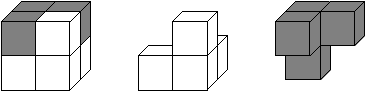
\includegraphics[width=0.9\textwidth]{two_colours.pdf}
\end{figure}

\begin{figure}
\center
\caption{Network of cubes, illustrating how the cubes fill space.}
\label{network_two_colours}
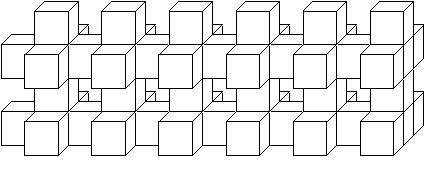
\includegraphics[width=0.9\textwidth]{network_two_colours.pdf}
\end{figure}

The question I want to investigate here is: can the same be done for three colours? What about
four or any number of colours, in fact? It turns out there are several ways of achieving a
division of space in this fashion, but none are as elegant as the two-colours division.


\section*{An irregular method}
With three colours we cannot quite use the same method as with two: select the cubes along
each of the three axes of a block of three by thee by three cubes. The number of cubes of
one colour would be 7 then, whereas we need 9 of each. But judiciously adding two of the
remaining cubes and we are done (Figure \ref{irregular_three_colours}).

The connectivity is guaranteed because the three cubes along each axis will touch the
three cubes of a neighbouring unit cell, in much the same way as for the case of two colours.

\begin{figure}
\center
\caption{Cubes in three colours -- "unit cell" for filling space.}
\label{irregular_three_colours}
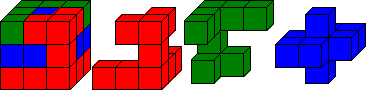
\includegraphics[width=0.9\textwidth]{irregular_three_colours.pdf}
\end{figure}

Since the unit cell is a cube, we can fill space in the same way as before, just put multiple
copies of the unit cube (in the same orientation) next to each other. The solution presented
here is only one of many, but the drawback is clearly that for each colour you need a different
configuration. Thus, it lacks something of the elegance of the two-colours division.

To get an impression of the number of possibilities:
\begin{itemize}
\item
We can fix one cube, in any location of the 27 cubes making up the unit cell, as it does not
matter which colour it gets. Therefore we need to assign colours to 26 cubes only.
\item
Using the rotational, reflexive and translational symmetries we can simply use that one
cube as the centre of the unit cell. That gives us 24 rotations and 24 reflections.
\item
For the first colour we need to select 8 cubes out of all 26 that are still colourless, leaving 18 cubes.
For the second colour we need to select 9 cubes out these 18 and for the third colour we have no
further choices.
\item
The total number $N$ of configurations of three colours is then:
\begin{eqnarray*}
    N &=& \binom{26}{8} \cdot \binom{18}{9} \\
      &=& 75957810500
\end{eqnarray*}
With the 48 symmetries (some configurations are symmetric, so that complicates matters) you
would end up with roughly $1.6 \cdot 10^9$ separate configurations. These all need to be examined
for connectivity.
\end{itemize}

If we limit ourselves to configurations like the chosen one, where you have three cubes in every direction
from one corner, we only need to select two more cubes for the first colour from the 13 uncoloured cubes and
two for the second colour out of 11. This gives:
\begin{eqnarray*}
    N_2 &=& \binom{13}{2} \cdot \binom{11}{2} \\
        &=& 4290
\end{eqnarray*}
\noindent which can be reduced by a factor 3 (rotational symmetry around the main diagonal joining the
two corners) to 1430.


\section*{Translate copies of a single layout}
An alternative is to design a layout that can be translated. One possibility is to extend
the layout from the two-colours unit cell, select two cubes with some care to make up for the
nine we need, and the result is a configuration like in Figure \ref{translated_three_colours}.

\begin{figure}
\center
\caption{Translated copies -- the "unit cell" is not depicted as a cube.}
\label{translated_three_colours}
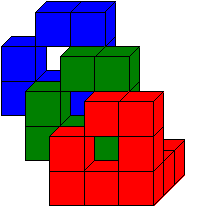
\includegraphics[width=0.4\textwidth]{translated_three_colours.pdf}
\end{figure}

It is not immediately clear, but the unit cell as shown fills space in the same way as
the ordinary blocks of 27 cubes from the first solution. And the configuration is the same
for all three colours. Extending this design to four or more colours will require selecting
the right cubes, though, just as in the first solution. Since the block for $n$ colours would
consist of $n^3$ cubes and the sides take up only $n+2(n-1 ~=~ 3n-2$ cubes, it will become
progressively more complicated to select the $n^2 - 3n + 2$ needed.


\section*{A systematic solution}
It turns out to be possible to divide space into three colours or actually $n$ colours
in a systematic way, such that the layouts for each colour is the same. Unfortunately,
we lose one of aspects of the two-colours solution: it is no longer isometric.

\begin{figure}
\center
\caption{Systematic configuration -- the "unit cell" two deep, not three.}
\label{systematic_three_colours}
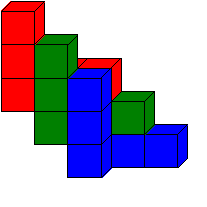
\includegraphics[width=0.4\textwidth]{systematic_three_colours.pdf}
\end{figure}

The idea is that each colour forms large holes in which the other colours can be fitted.
Isolating a single colour, the configuration is that of Figure \ref{systematic_configuration}.

\begin{figure}
\center
\caption{Systematic configuration -- isolating a single colour.}
\label{systematic_configuration}
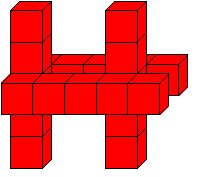
\includegraphics[width=0.4\textwidth]{systematic_configuration.pdf}
\end{figure}

While not isometric like the two-colours solution, it does have an
elegant structure: you can distinguish two subsets of cubes, one
consisting of vertical stacks of cubes and the other of horizontal
rows. The other colours follow the same simple pattern, only shifted
in the horizontal and vertical direction. The unit cell is $3 \times 3 \times 2$
instead of $3 \times 3 \times 3$, as with the other solutions.

\section*{Other dimensions}
Most likely you can extend this type of division to other dimensions as well,
although it is very difficult to visualise such divisions. For two dimensions
there is a peculiar problem: periodic solutions, like the
ones we have seen here with a finite unit cell, seem impossible. One alternative
is a spiral-like design. You can easily see that a periodic solution is not
possible (though the line of reasoning hardly consitutes a rigorous proof):
If you could construct a periodic solution, then there would be a chain of squares
all of one colour that stretches from one end of the plane to the other. The chain
may be very complicated in shape, but essentially it would divide the plane into
at least two parts. So, it would not be possible for another unbroken chain to fill
the rest of the plain.

\begin{figure}
\center
\caption{Examples of spirals covering the plane.}
\label{squares_spiralling}
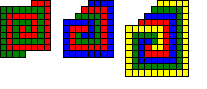
\includegraphics[width=0.8\textwidth]{squares_spiralling.pdf}
\end{figure}


\section*{Spiral solutions in two dimensions}
To get an idea of the spiral-like solutions consider the picture with spirals of
two, three and four different colours (figure \ref{squares_spiralling}). The central part is where the pattern is
not uniform, but the overall pattern is uniform in the sense that all colours
occupy an equal number of squares and there is no preference for one direction
or the other.

\begin{figure}
\center
\caption{Systematic set-up for an arbitrary number of colours.}
\label{systematic_spiralling}
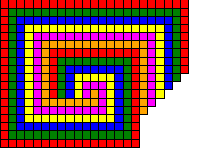
\includegraphics[width=0.8\textwidth]{systematic_spiralling.pdf}
\end{figure}

There are endless possibilities to arrange the spirals, like a central region where the coloured
chains follow a zig-zag pattern before settling on a spiral, the solutions shown are but a
single possibility. It is even possible to set up this simple type in a systematic way,
using any number of colours, as shown in Figure \ref{systematic_spiralling}: start with a row
of squares with all the colours and add a square with the colour at the end, going round the row (orange in the figure).
Then the last but one colour (magenta) can form a spiral going around that one and so on.

\end{document}


